% version 1.00, date 07/03/16, auteur Mélissa Bignoux

\documentclass[asi]{picInsa}

%Pour le schéma d'architecture
\usepackage{etex}
\usepackage{tikz}
\usetikzlibrary{shapes,arrows,chains,backgrounds,fit}
%FIN Pour le shéma d'architecture

\DeclareGraphicsRule{*}{pdf}{*}{}
\usepackage{pdfpages}
\usepackage{vocabulaireUnipik}




\setcounter{secnumdepth}{4}
\setcounter{tocdepth}{4}
\newcommand{\ligneMaj}[3] {
	\rowcolor[gray]{0.55} \textbf{\textit{#1}} & #2  &  #3\\
	\hline
}
\newcommand{\ligneSup}[3] {
	\rowcolor[gray]{0.65} |\textunderscore \textbf{\textit{#1}} & #2  &  #3\\
	\hline
}
\newcommand{\ligneMed}[3] {
	\rowcolor[gray]{0.75} \hspace{0.25cm} |\textunderscore #1  & #2 & #3 \\
	\hline
}
\newcommand{\ligneSub}[3] {
	\rowcolor[gray]{0.85}  \hspace{0.5cm} |\textunderscore #1 & #2 & #3\\
	\hline
}
\newcommand{\ligneSubSub}[3] {
	\rowcolor[gray]{0.95}  \hspace{0.75cm} |\textunderscore #1 & #2 & #3\\
	\hline
}
\newcommand{\ligneTache}[3] {
	\hspace{1.00cm} |\textunderscore #1 & #2 & #3\\
	\hline
}
\title{\DCP{}}
\author{\Florian{}, \Kafui{}, \Melissa{}, \Julie{}, \Mathieu{}} %à changer


\titreGeneral{\DCP}
\sousTitreGeneral{\nomEquipe}
\titreAcronyme{\DCPCourt}

\titreDetaille{\DCPCourt\_D\_\nomEquipe\_l2}
\referenceVersion{\DCPCourt\_D\_\nomEquipe\_\versionPrive}
\auteurs{\Melissa{} \& \Florian{} \& \Michel{}}
\destinataires{\nomEquipe}
\resume{Le présent document contient la présentation du \DCP{} \nomEquipe.}
\motsCles{\DCPCourt{}}
\natureDerniereModification{Création}
\modeDiffusionControle{}

\begin{document}

\couverture{}

 \informationsGenerales{}
% version 1.00, date 29/02/16, auteur Michel Cressant
\begin{pagesService}
	\begin{historique}
		% nouvelles versions à rajouter AU-DESSUS en recopiant les lignes suivantes et en les modifiant :
		\unHistorique{1.00}{02/02/2016}{\Michel}{Création}{Toutes}

	\end{historique}

%        \begin{suiviDiffusions}
%
%            % On place ici les diffusions
%        	\unSuivi{1.00}{}{\nomEquipe{}}
%          
%          
%        \end{suiviDiffusions}

%%Signataires
        \begin{signatures}
	   \uneSignature{Vérificateur}{\RRS}{\Matthieu{}}{17/03/2016}{PGPic}
       \uneSignature{Validateur}{\CP{}}{\Sergi}{}{PGPic}
        \end{signatures}
	
	

	
	
\end{pagesService}


\tableofcontents

\setcounter{chapter}{0}


\chapter*{Introduction}
\label{intro}
% version 1.01 Date 24/03/2016	Auteur Mathieu Medici

\section*{Objet}
L'objectif de ce document est de présenter les principes et les procédures nécessaires à la mise en œuvre de la gestion des configurations prévue par la norme \isoNeufMilleUn.

\section*{Définition}

Le présent document établit les règles et la structure de la gestion des configurations qui doivent être suivies pendant toute la durée du \picCourt. Il contient :
\begin{itemize}
\item les règles de nommage;
\item la description des différents référentiels;
\item les règles spécifiques de \nomEquipe{};
\item la description de l'administration des configurations;
\item la description de la maîtrise des documents;
\item la description de la maîtrise des enregistrements;
\item les règles d'archivage.
\end{itemize}



\chapter{Cas d'utilisation}
\label{casUtilisation}
% version 1.00, date 20/02/16, auteur Michel Cressant
Ce chapitre décrit les différents cas d'utilisation pour chaque fonctionnalité.


\section{Fonctionnalité 8}
Ce paragraphe décrit les cas d'utilisation concernant la fonctionnalité 8 soit la géolocalisation. \\

La figure suivante (figure \ref{diagrammeCasUtilisation8}) indique les cas d'utilisation pour la géolocalisation.
\begin{figure}[H]
	\centering
	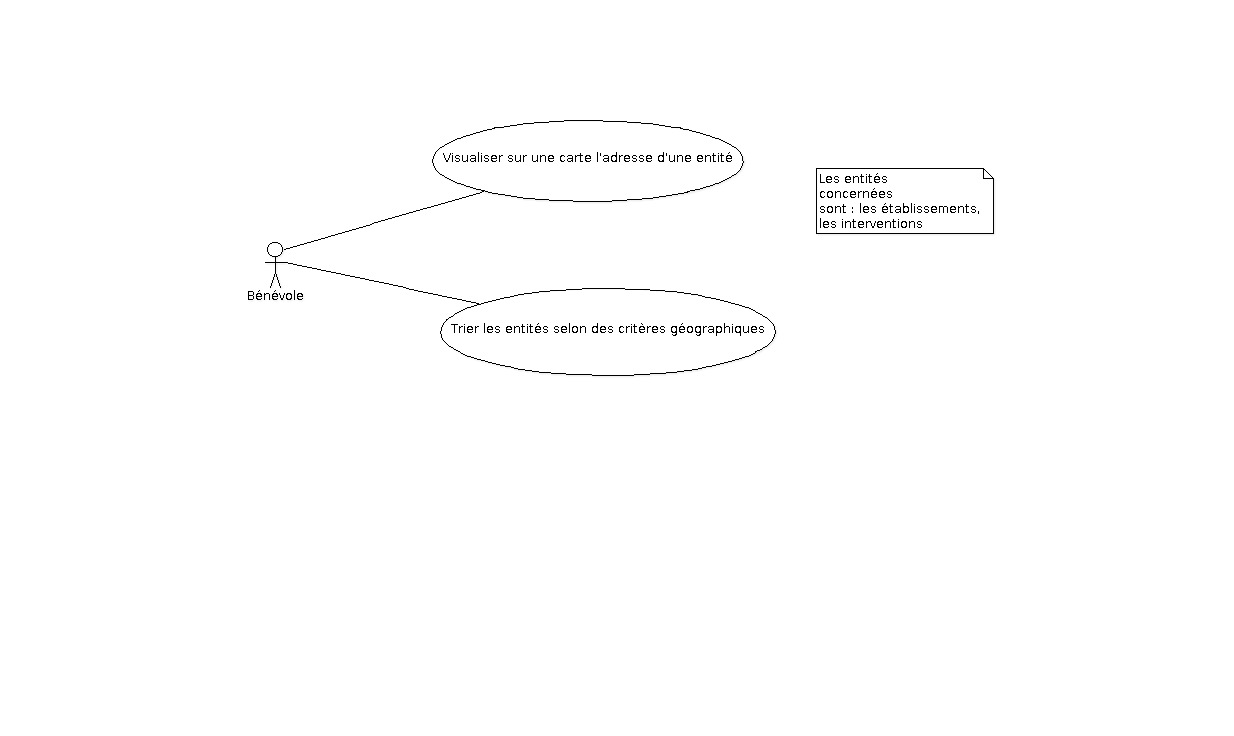
\includegraphics[scale=0.40]{casDUtilisation/images/fonctionnalite8Geolocalisation.png}
	\caption{Cas d'utilisation~: Géolocalisation }
	\label{diagrammeCasUtilisation8}
\end{figure}

\section{Fonctionnalité 9}
Ce paragraphe décrit les cas d'utilisation concernant la fonctionnalité 9 soit l'attribution de frimousse. \\

La figure suivante (figure \ref{diagrammeCasUtilisation9}) indique les cas d'utilisation pour l'attribution de frimousse.
\begin{figure}[H]
	\centering
	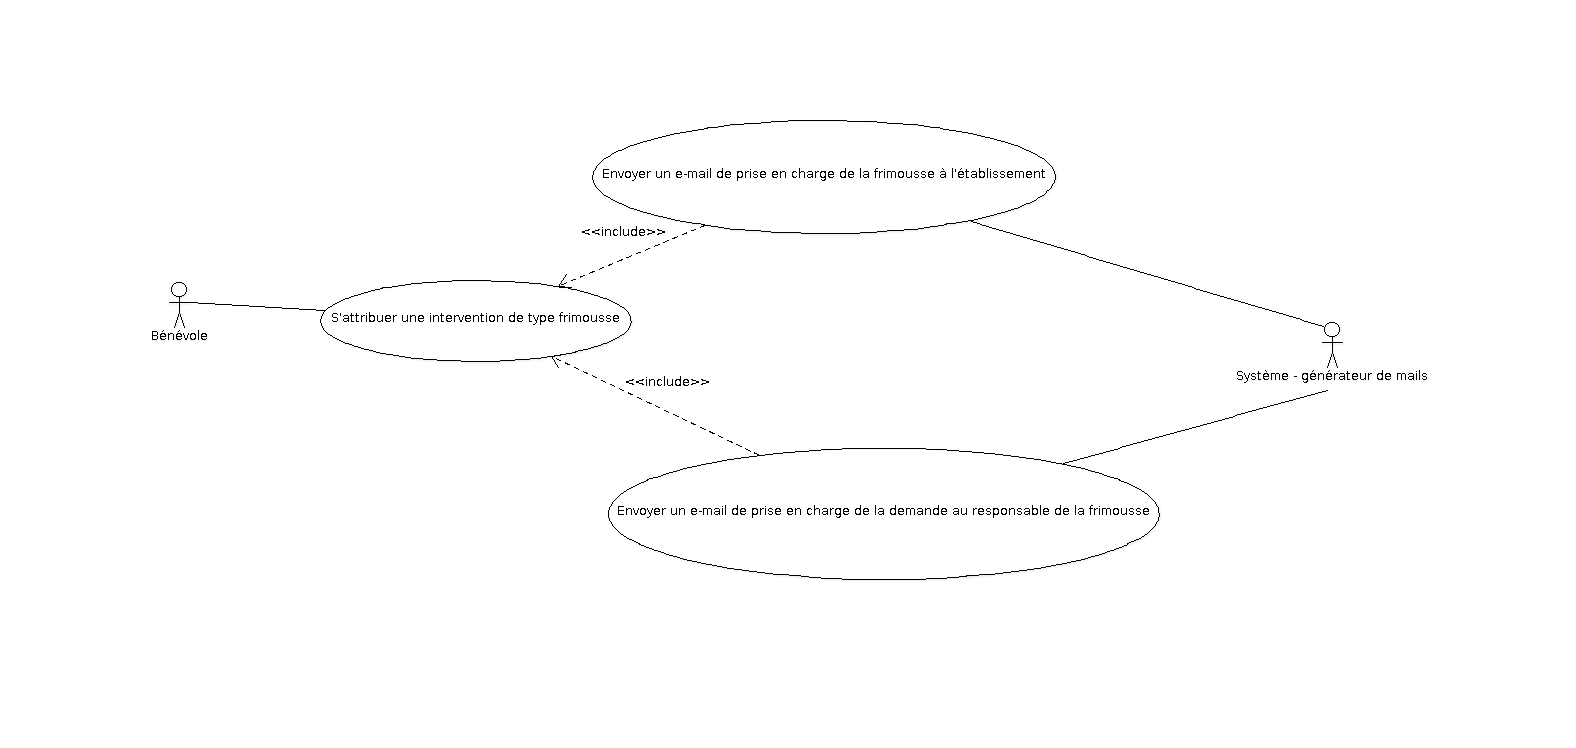
\includegraphics[scale=0.35]{casDUtilisation/images/fonctionnalite9Attribution.png}
	\caption{Cas d'utilisation~: Attribution de frimousse }
	\label{diagrammeCasUtilisation9}
\end{figure}

\section{Fonctionnalité 10}
Ce paragraphe décrit les cas d'utilisation concernant la fonctionnalité 10 soit la gestion des ventes. \\

La figure suivante (figure \ref{diagrammeCasUtilisation10}) indique les cas d'utilisation pour l'attribution de frimousse.
\begin{figure}[H]
	\centering
	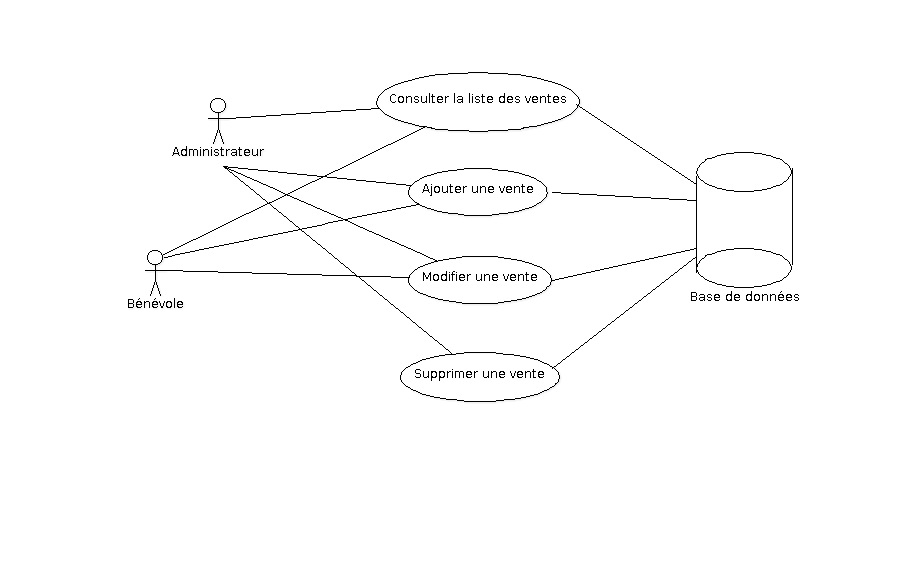
\includegraphics[scale=0.40]{casDUtilisation/images/fonctionnalite10Vente.png}
	\caption{Cas d'utilisation~: Gestion des ventes }
	\label{diagrammeCasUtilisation10}
\end{figure}


\chapter{Maquettes}
\label{maquettes}
% version 1.00, date 12/11/16, auteur Kafui Atanley
Ce chapitre présente les maquettes pour chaque fonctionnalité pour chaque fonctionnalité additionnelle du lot 3 par rapport au lot 2.


\section{Fonctionnalité 8}
Ce paragraphe décrit les maquettes concernant la fonctionnalité 8 soit la géolocalisation. \\

La figure suivante \ref{maquette8-1} montre la maquette d'une fiche descriptive d'une entité possédant une adresse. Un espace devra être réservé pour afficher la location de l'entité comme visible sur la fmaquette.
\begin{figure}[H]
	\centering
	\includegraphics[scale=0.40]{images/maquettes/fonctionnalite9Geolocalisation.png}
	\caption{Maquette~: Fiche descriptive d'une entité possédant une adresse}
	\label{maquette8-1}
\end{figure}
La figure suivante \ref{maquette8-2} présente la maquette des filtres de tri attendus sur la géolocalisation dans les pages permettant de lister les entités.
\begin{figure}[H]
	\centering
	\includegraphics[scale=0.40]{images/maquettes/fonctionnalite9Filtre.png}
	\caption{Maquette~: Modèle de filtre attendues dans les liste de tri}
	\label{maquette8-2}
\end{figure}

\section{Fonctionnalité 9}
Ce paragraphe décrit les maquettes concernant la fonctionnalité 9 soit l'attribution de frimousse. \\

La figure suivante montre l'email type de prise en charge d'une intervention de type frimousse.

La figure suivante montre la maquette de l'interface pour la prise en charge d'une intervention de type frimousse. L'utilisateur pourra s'attribuer une intervention de type frimousse via la liste d'intervention ou via la fiche descriptive de cette intervention.


\section{Fonctionnalité 10}
Ce paragraphe décrit les maquettes concernant la fonctionnalité 10 soit la gestion des ventes. \\

La figure suivante montre la maquette \ref{maquette10-5} de la page permettant d'ajouter une vente .
\begin{figure}[H]
	\centering
	\includegraphics[scale=0.40]{images/maquettes/fonctionnnalite10AjouterVente.png}
	\caption{Maquette~: Ajouter une vente}
	\label{maquette10-5}
\end{figure}

La figure suivante \ref{maquette10-3} montre la maquette de la page de la fiche descriptive d'une vente.
\begin{figure}[H]
	\centering
	\includegraphics[scale=0.40]{images/maquettes/fonctionnnalite10ConsulterVente.png}
	\caption{Maquette~: Consulter la fiche descriptive d'une vente}
	\label{maquette10-3}
\end{figure}

La figure suivante \ref{maquette10-4} Listing des ventes montre la maquette de la page permettant d'effectuer le listing des ventes.
\begin{figure}[H]
	\centering
	\includegraphics[scale=0.40]{images/maquettes/fonctionnalite10Ventes.png}
	\caption{Maquette~: Listing des ventes}
	\label{maquette10-4}
\end{figure}

La figure suivante \ref{maquette10-4} Listing des ventes montre la maquette de la page permettant d'effectuer le listing des ventes.

Il est possible de supprimer une vente à partir de la fiche descriptive d'une vente 




\chapter{Diagramme de séquence système}
\label{diagrammeSequenceSysteme}
% version 1.00, date 20/02/16, auteur Michel Cressant
\begin{figure}[H]
\centering 
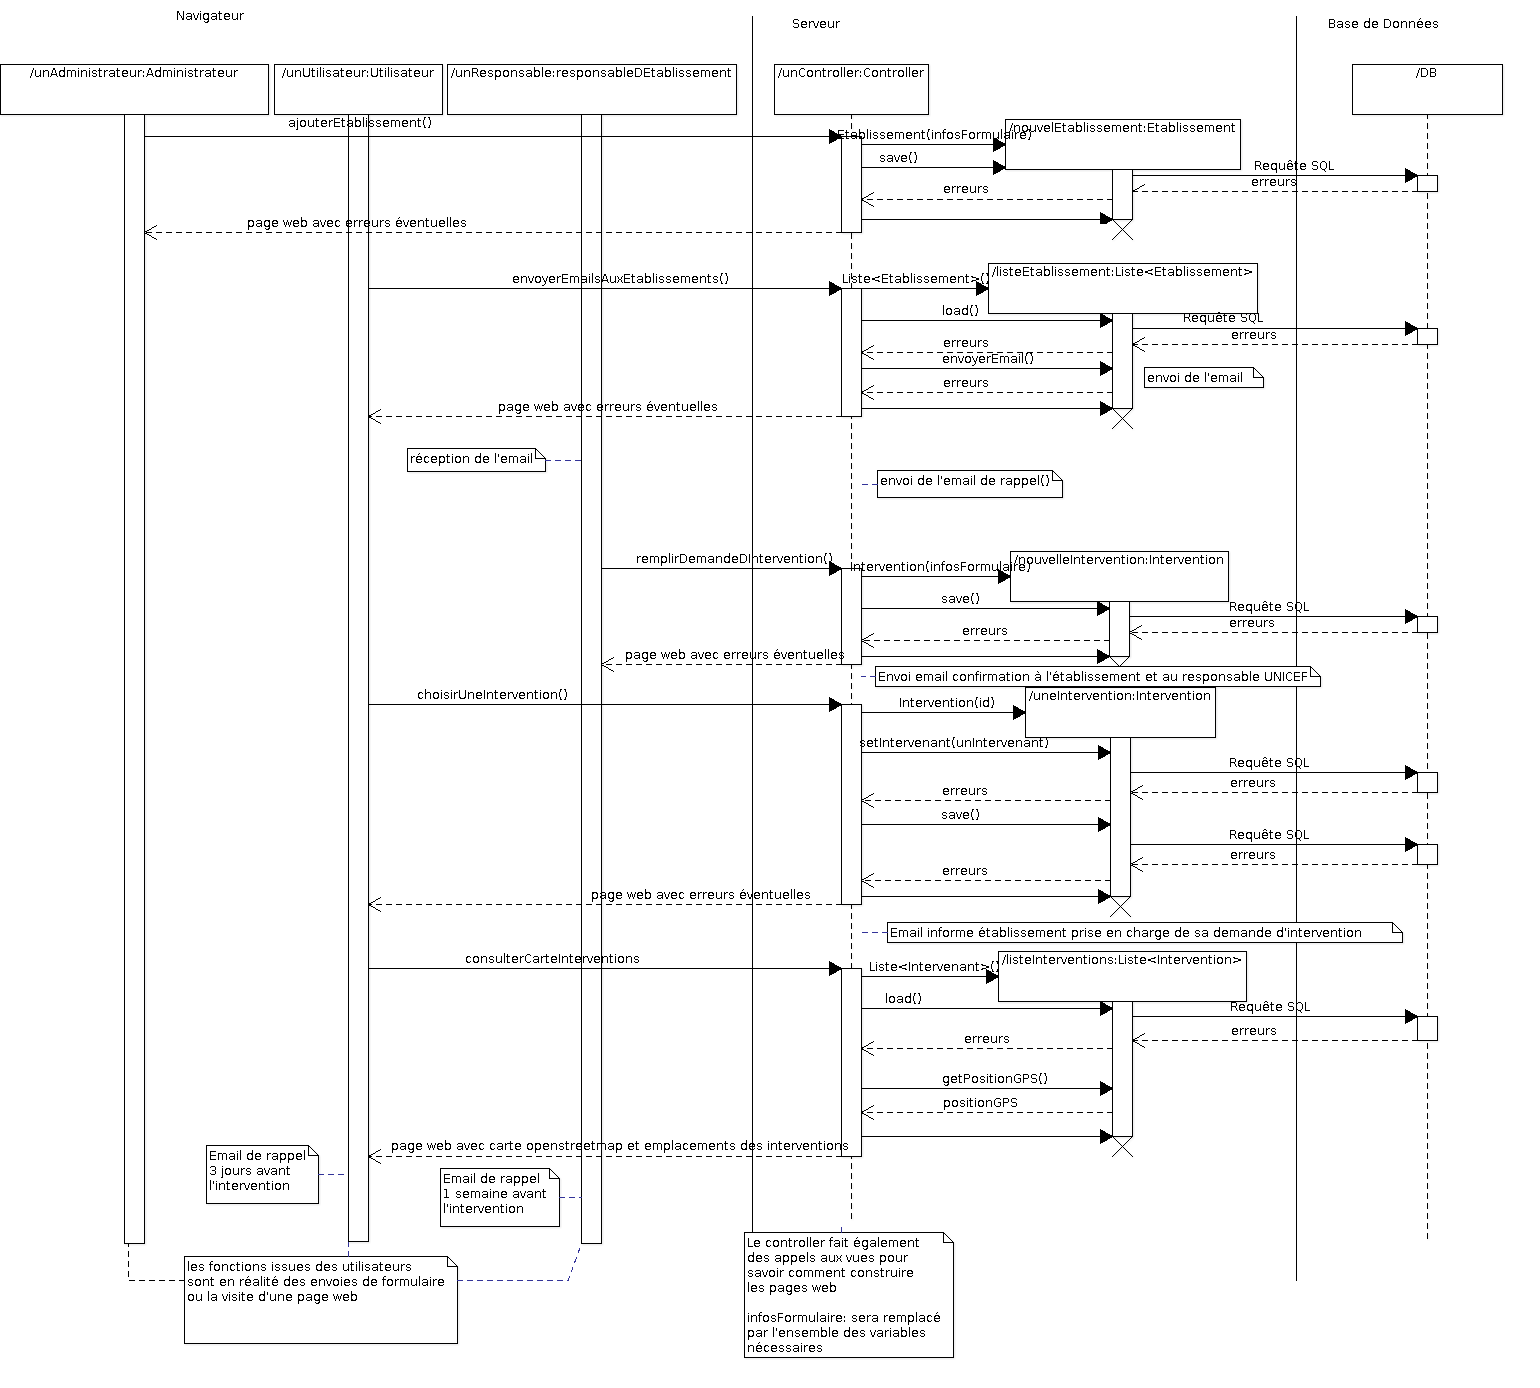
\includegraphics[scale=0.34]{images/diagrammeSequenceSysteme/diagrammeSequence.png}
\caption{Diagramme de séquence système}
\label{diagrammeDeSequenceSysteme}
\end{figure}

Ce diagramme (figure \ref{diagrammeDeSequenceSysteme}) présente le diagramme de séquence système du lot 2 de notre projet. \\
Comme présenté sur la figure, l'administrateur pourra ajouter un établissement à la base de données. Cette dernière action peut se décomposer en plusieurs étapes : 
\begin{itemize}
	\item l'administrateur clique sur ajouter un établissement;
	\item l'administrateur entre les données de l'établissement dans le formulaire;
	\item le contrôleur récupère les informations du formulaire et met à jour la base de données;
	\item si une erreur apparaît, une page d'erreur est renvoyée à l'administrateur.\\
\end{itemize}


La création de profil s'effectuera de la même manière que l'ajout d'un établissement à la base de données, seules les informations demandées dans les formulaires diffèreront.\\



Une autre des fonctionnalités de notre lot 2 est l'envoi d'e-mails aux établissements. Celle-ci peut également se décomposer en diférentes étapes : 
\begin{itemize}
	\item l'utilisateur déclenche l'envoi d'e-mails aux établissements; 
	\item le contrôleur récupère la liste des adresses e-mails des établissements;
	\item le contôleur envoie à cette liste d'adresses un e-mails un courriel type afin de proposer aux établissements des interventions pour sensibiliser les enfants à différents thèmes. Cet e-mail contiendra un lien vers un formulaire qui permettra aux établissements d'effectuer des demandes d'intervention;
	\item si une erreur se produit, une page d'erreur sera renvoyée à l'utilisateur;
	\item si l'établissement ne remplit le formulaire de demande d'interventions après un certain temps, un e-mail de rappel sera envoyé aux établissements. \\
\end{itemize}   


L'étape suivante est le remplissage du formulaire par l'établissement demandeur. A chaque demande d'interventions:  
\begin{itemize}
	\item chaque intervention de la demande de l'établissement sera ajouté à la base de données;
	\item un e-mail de confirmation de demande d'interventions sera envoyé à l'établissement, lui permettant également d'annuler cette dernière;
	\item un e-mail d'information sera envoyé aux responsables d'activitéde l'UNICEF;
	\item en cas d'erreur, une page d'erreur sera renvoyée à l'utilisateur.\\
\end{itemize}


Lorsque la base de données contiendra des interventions, un bénévole pourra choisir une intervention et se l'attribuer. Cette action donnera une valeur à l'intervenant de l'intervention dans la base de données. Si une erreur se produit, une page d'erreur sera renvoyée. A chaque attribution d'une intervention à un intervenant, un e-mail d'information de prise en charge de la demande sera envoyé à l'établissement et au reponsable de l'activité de l'UNICEF. \\

Notre produit permettra également de visualiser une carte présentant toutes les interventions pour une date et un moment entrés par l'utilisateur. En cas d'erreur, une page d'erreur sera renvoyée à l'utilisateur. \\

Le plaideur responsable d'une intervention pourra mettre à jour les informations des interventions desquelles il est reponsable. Cela entrainera une mise à jour des interventions modifiées dans la base de données. Après chaque mise à jour, un e-mail informant l'établissement des mises à jour sera envoyée. \\

Une semaine avant chaque intervention, un e-mail sera envoyé à l'établissement concerné.  
Trois jours avant chaque intervention, un e-mail sera envoyé au plaideur responsable de l'intervention. 




\chapter{Diagramme d'activité de navigation}
\label{diagrammeNavigation}
% version 1.00, date 10/11/16, auteur Kafui Atanley
Ce chapitre décrit la carte de navigation sous la forme d'un diagramme d'état-transissions.

La figure suivante (figure \ref{diagrammeEtatTrans}) présente la carte de navigation sous la forme d'un diagramme d'état-transissions.
\begin{figure}[H]
	\centering
	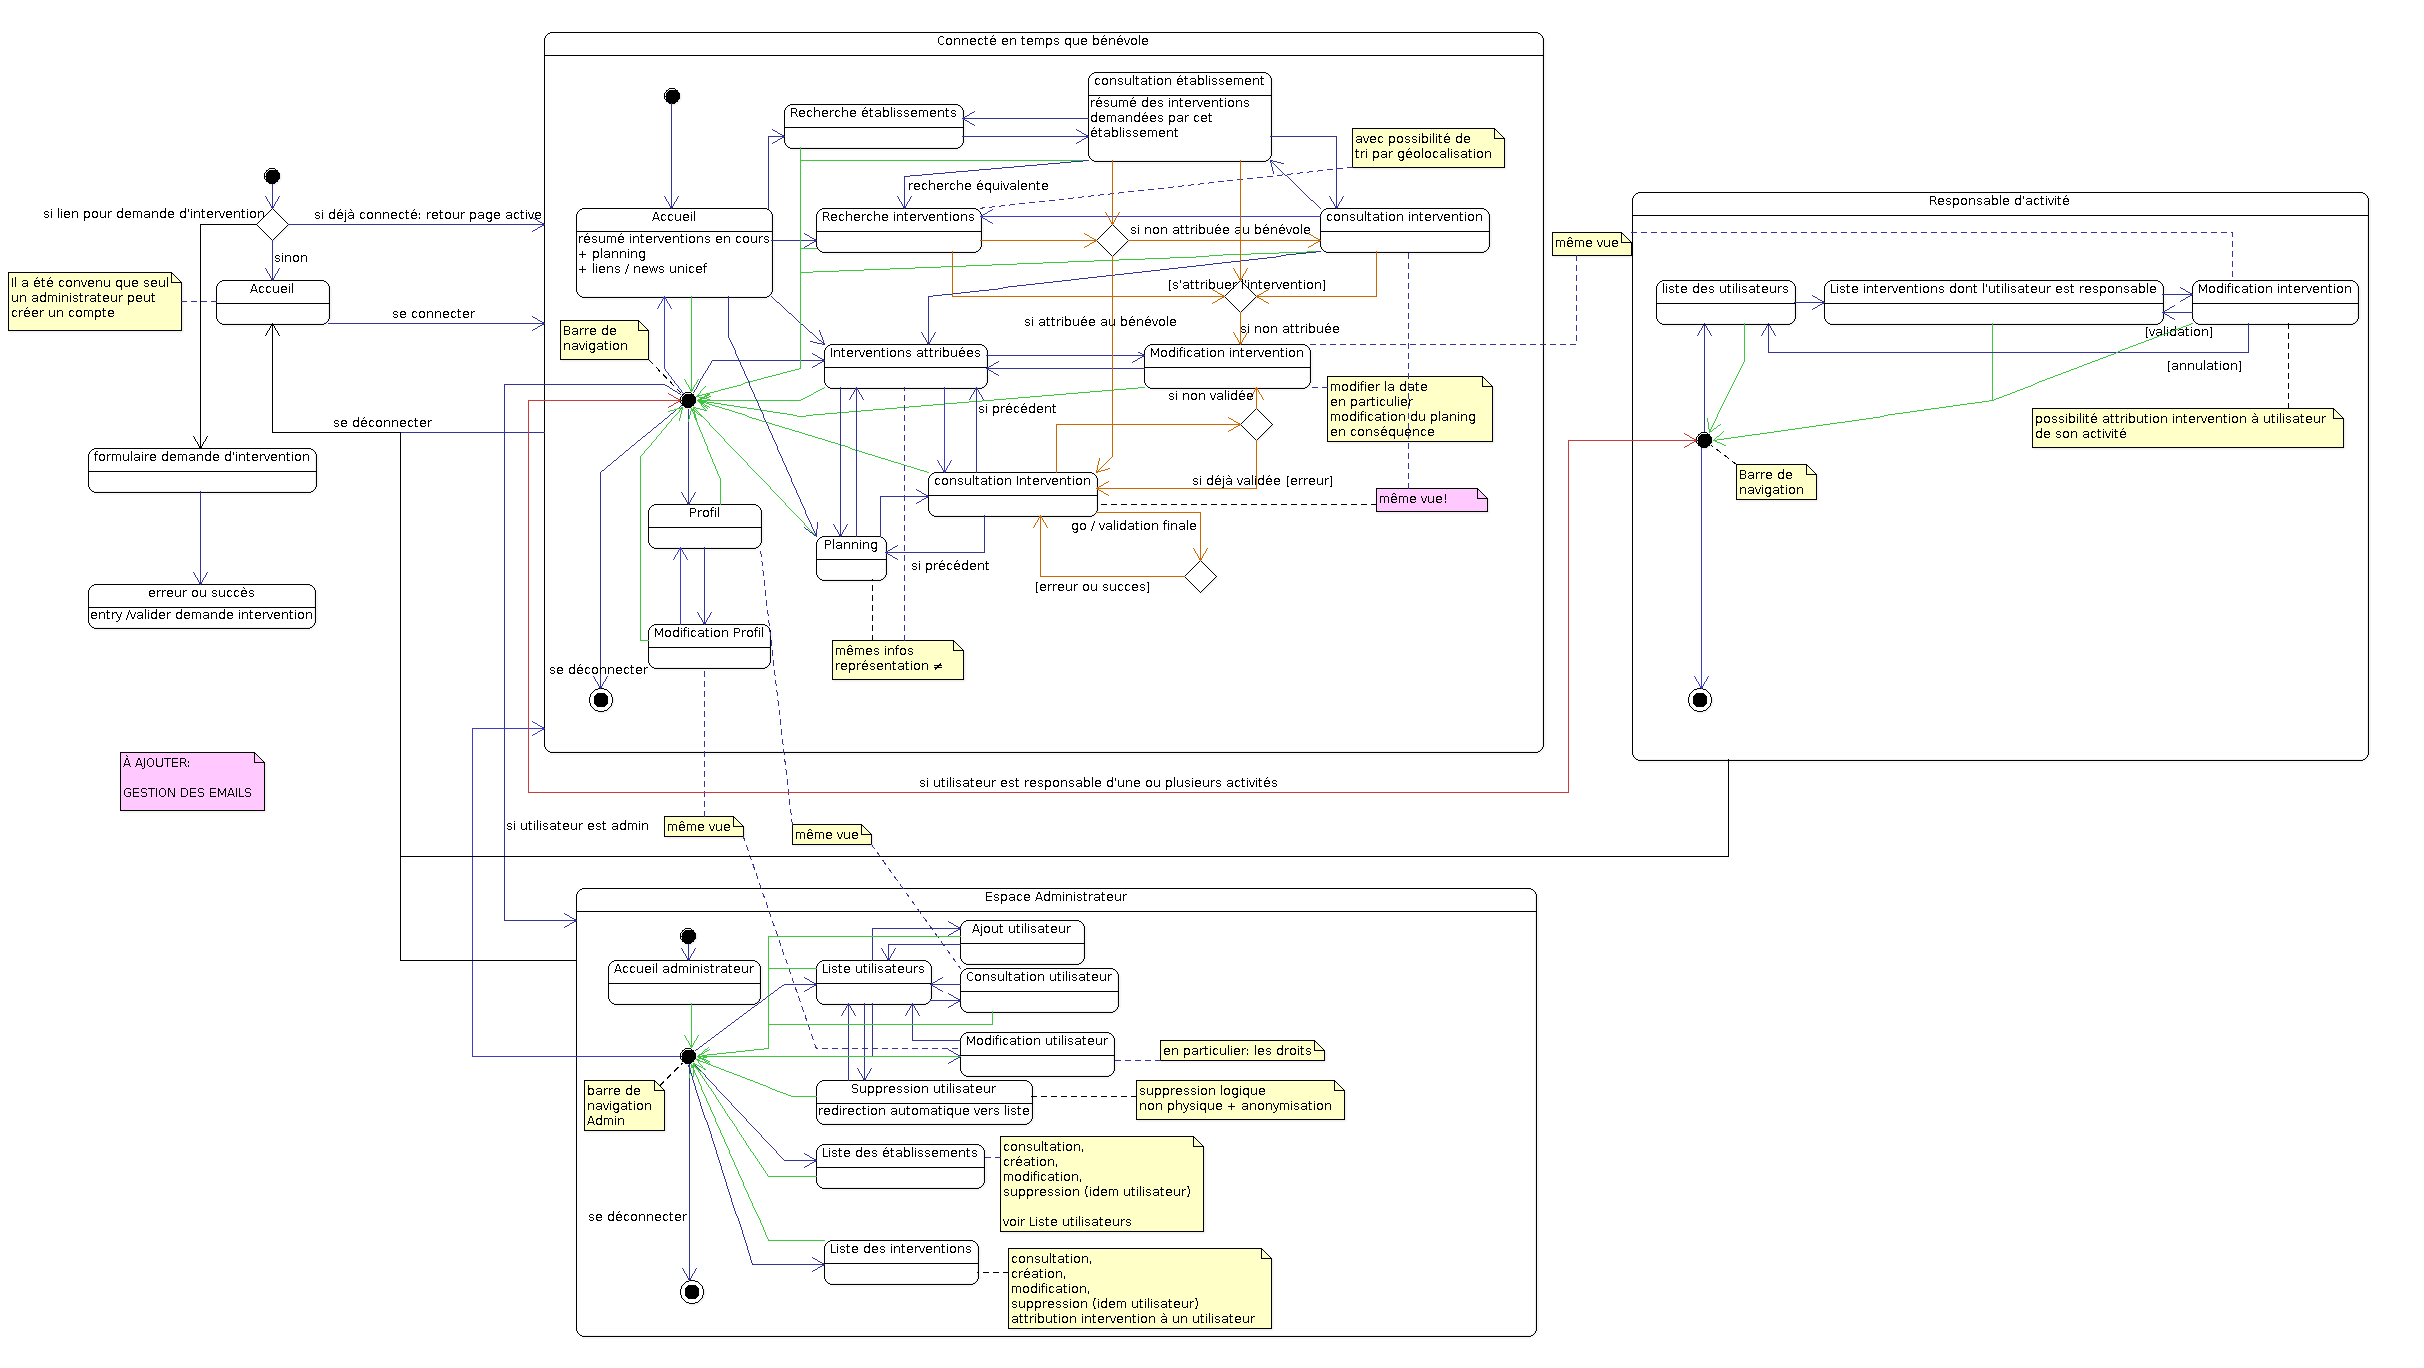
\includegraphics[scale=0.20]{images/diagrammeEtatsTransitions/carteDeNavigation.png}
	\caption{Carte de navigation (diagramme d'état-transissions)}
	\label{diagrammeEtatTrans}
\end{figure}


\chapter{Diagrammes d'intéraction}
\label{diagrammeInteraction}
% version 1.00, date 10/10/16, auteur Kafui Atanley
Ce chapitre décrit les différents diagrammes d'intéraction.
\section{Lot 2}
\subsection{Fonctionnalité 1}
Ce paragraphe décrit les diagrammes d'intéraction concernant la fonctionnalité 1. \\

La figure suivant (figure \ref{diagrammeInteraction1}) indique le déroulement de la création, la modification et la suppression d'un bénévole par un administrateur.
\begin{figure}[H]
	\centering
	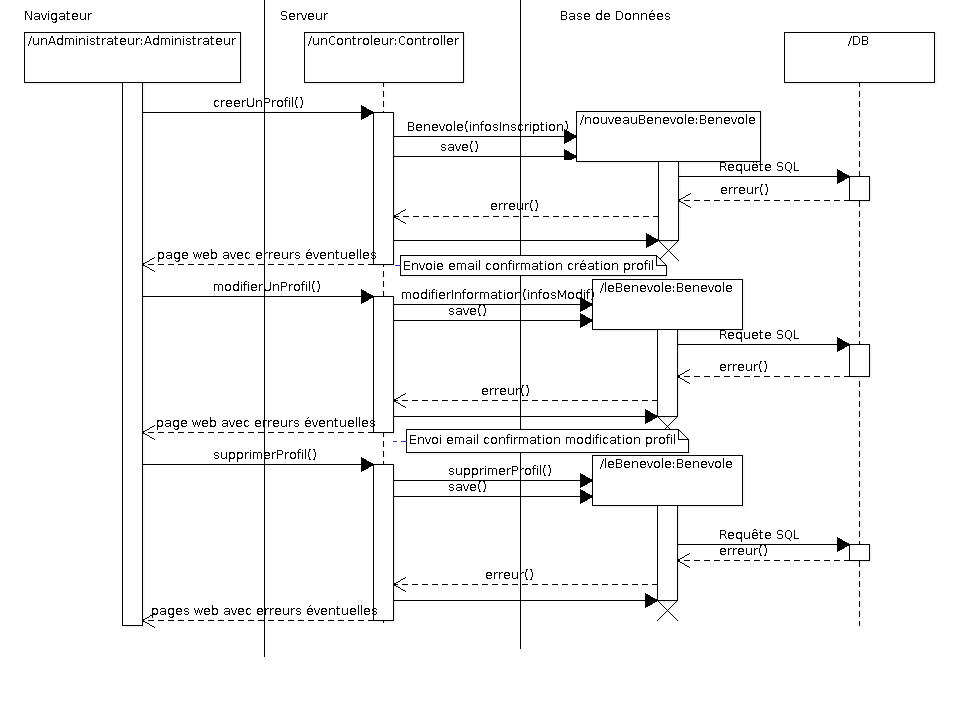
\includegraphics[scale=0.57]{../../lot2/DCP/images/diagrammesInteraction/01_diagrammeInteractionF1.png}
	\caption{Diagramme d'intéraction~: Création, modification, suppression d'un bénévole par un administrateur}
	\label{diagrammeInteraction1}
\end{figure}

La figure suivante (figure \ref{diagrammeInteraciton2}) indique le déroulement de la connexion et la déconnexion d'un bénévole.
\begin{figure}[H]
	\centering
	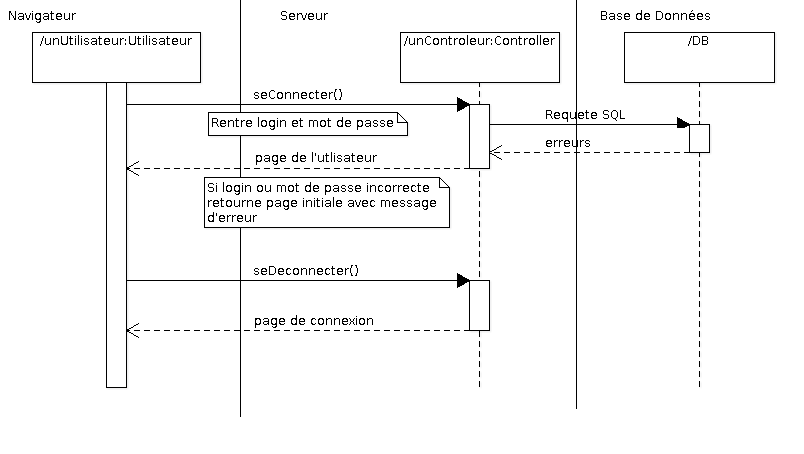
\includegraphics[scale=0.65]{../../lot2/DCP/images/diagrammesInteraction/02_diagrammeInteractionF1.png}
	\caption{Diagramme d'intéraction~: Connection et déconnection d'un utilisateur}
	\label{diagrammeInteraciton2}
\end{figure}

\subsection{Fonctionnalité 2}
Ce paragraphe décrit le diagramme d'intéraction concernant la fonctionnalité 2. \\

La figure suivante (figure \ref{diagrammeInteraction3}) indique le déroulement de la création, la modification et la suppression d'un établissement par un administrateur.
\begin{figure}[H]
	\centering
	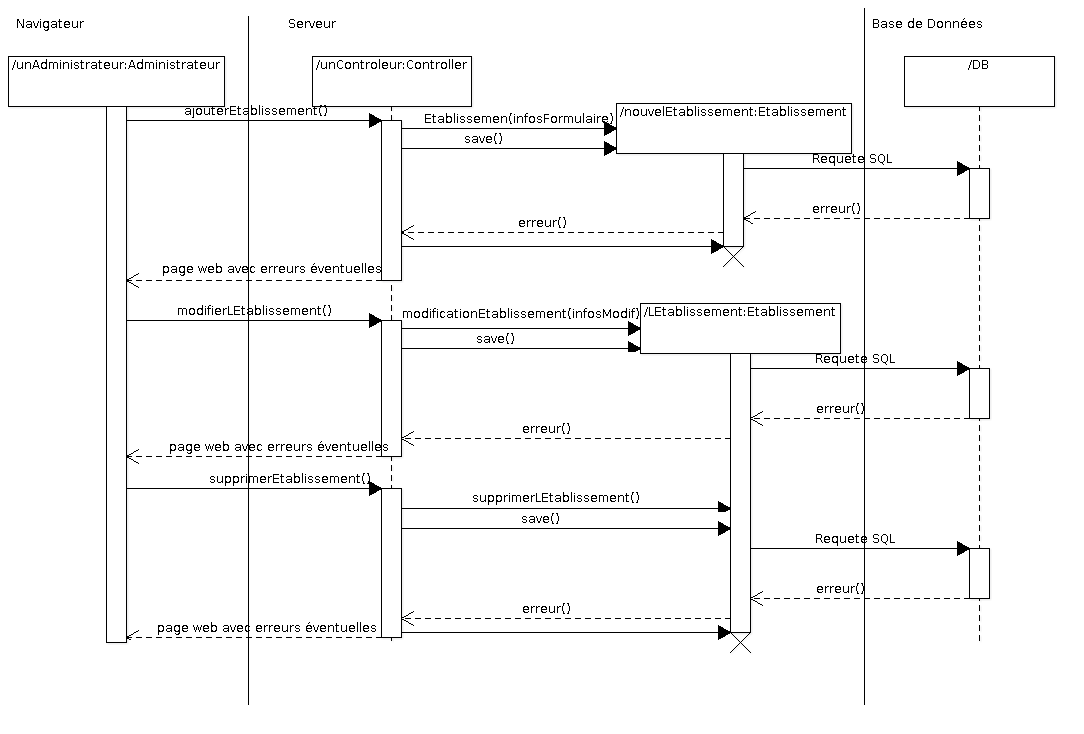
\includegraphics[scale=0.5]{../../lot2/DCP/images/diagrammesInteraction/03_diagrammeInteractionF2.png}
	\caption{Diagramme d'intéraction~: Création, modification, suppression d'un établissement par un administrateur}
	\label{diagrammeInteraction3}
\end{figure}

\subsection{Fonctionnalité 3}
Ce paragraphe décrit le diagramme d'intéraction concernant la fonctionnalité 3. \\

La figure suivante (figure \ref{diagrammeInteraction4}) indique le déroulement de l'envoi du formulaire de demande d'intervention aux établissements.
\begin{figure}[H]
	\centering
	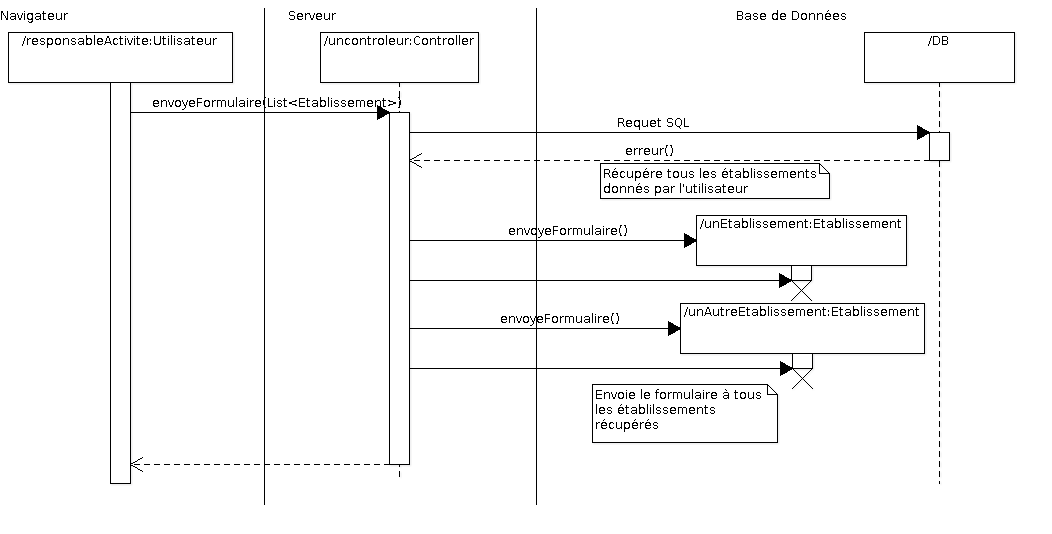
\includegraphics[scale=0.5]{../../lot2/DCP/images/diagrammesInteraction/04_diagrammeInteractionF3.png}
	\caption{Diagramme d'intéraction~: Envoye du formulaire à un ensemble d'établissement}
	\label{diagrammeInteraction4}
\end{figure}

\subsection{Fonctionnalité 4}
Ce paragraphe décrit les diagramme d'intéraction concernant la fonctionnalité 4. \\

La figure suivante (figure \ref{diagrammeInteraction5}) indique le déroulement du remplissage du formualaire de demande d'intervention.
\begin{figure}[H]
	\centering
	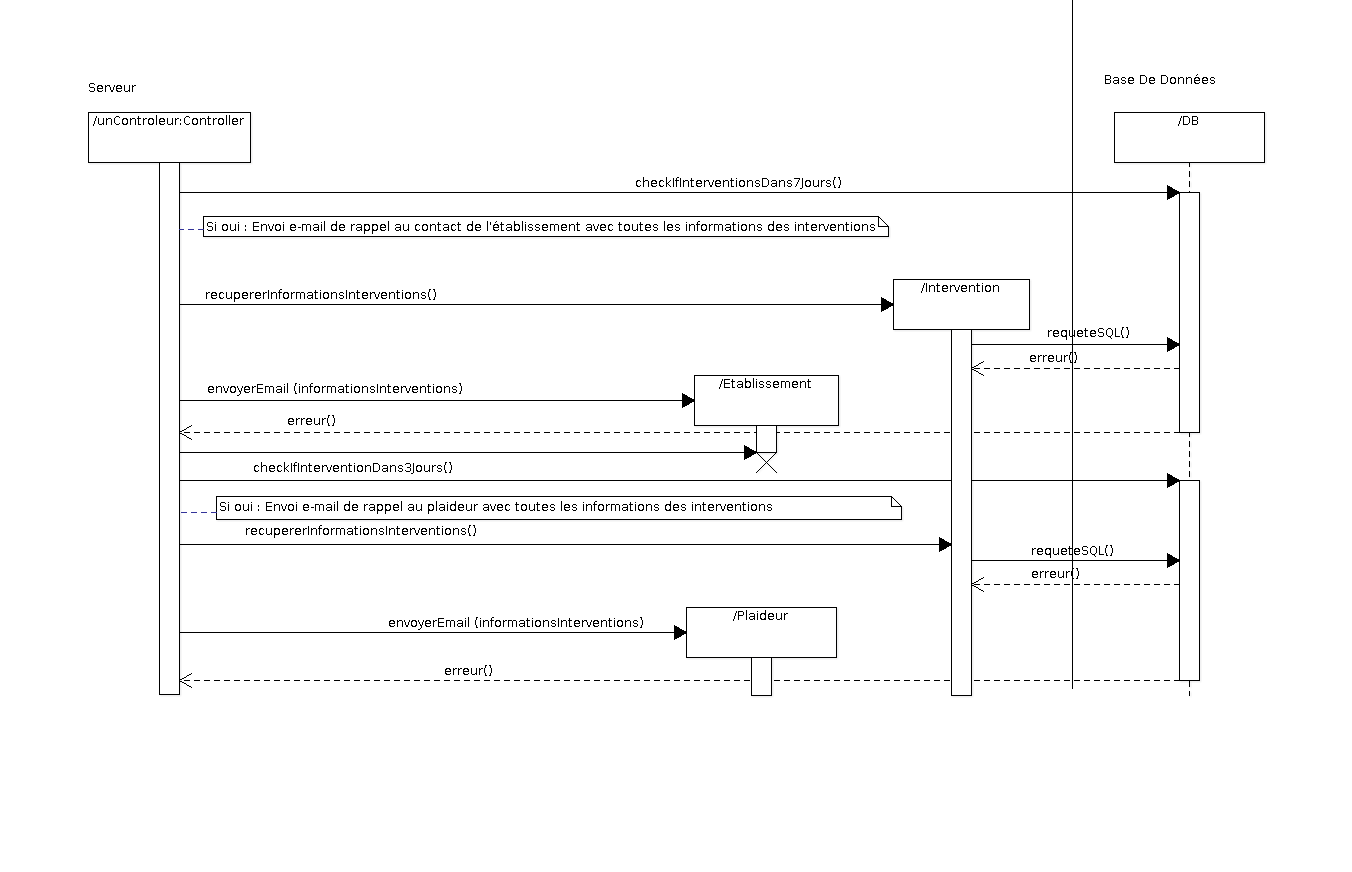
\includegraphics[scale=0.5]{../../lot2/DCP/images/diagrammesInteraction/05_diagrammeInteractionF4.png}
	\caption{Diagramme d'intéraction~: Replissage du formulaire}
	\label{diagrammeInteraction5}
\end{figure}


La figure suivante (figure \ref{diagrammeInteraction6}) indique le déroulement de l'annulation d'une demande d'intervention.
\begin{figure}[h]
	\centering
	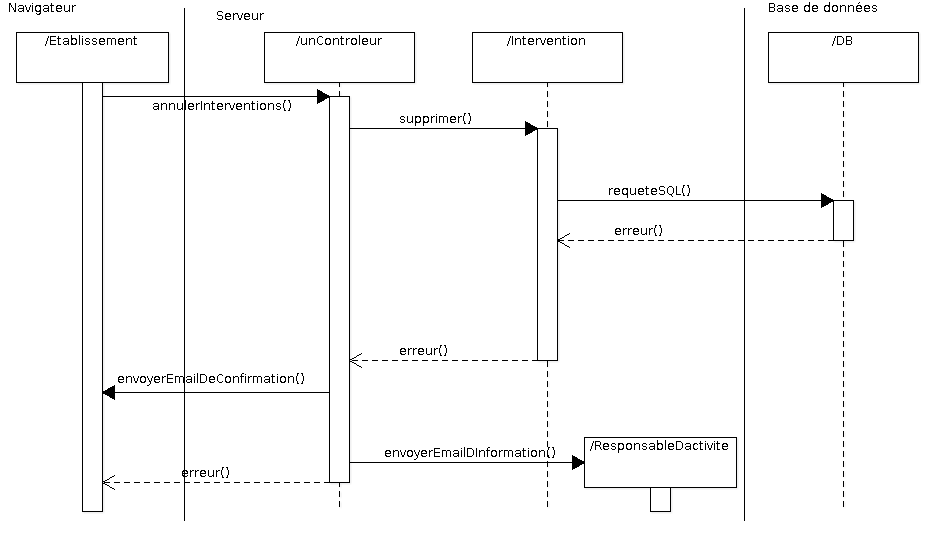
\includegraphics[scale=0.5]{../../lot2/DCP/images/diagrammesInteraction/06_diagrammeInteractionF4.png}
	\caption{Diagramme d'intéraction~: Annulation d'une demande d'intervention}
	\label{diagrammeInteraction6}
\end{figure}

\subsection{Fonctionnalité 5}
Ce paragraphe décrit le diagramme d'intéraction concernant la fonctionnalité 5. \\

La figure suivante (figure \ref{diagrammeInteraction7}) indique le déroulement de la géolocalisation des interventions ainsi que l'affectation d'un plaideur à celles ci. \\
\begin{figure}[H]
	\centering
	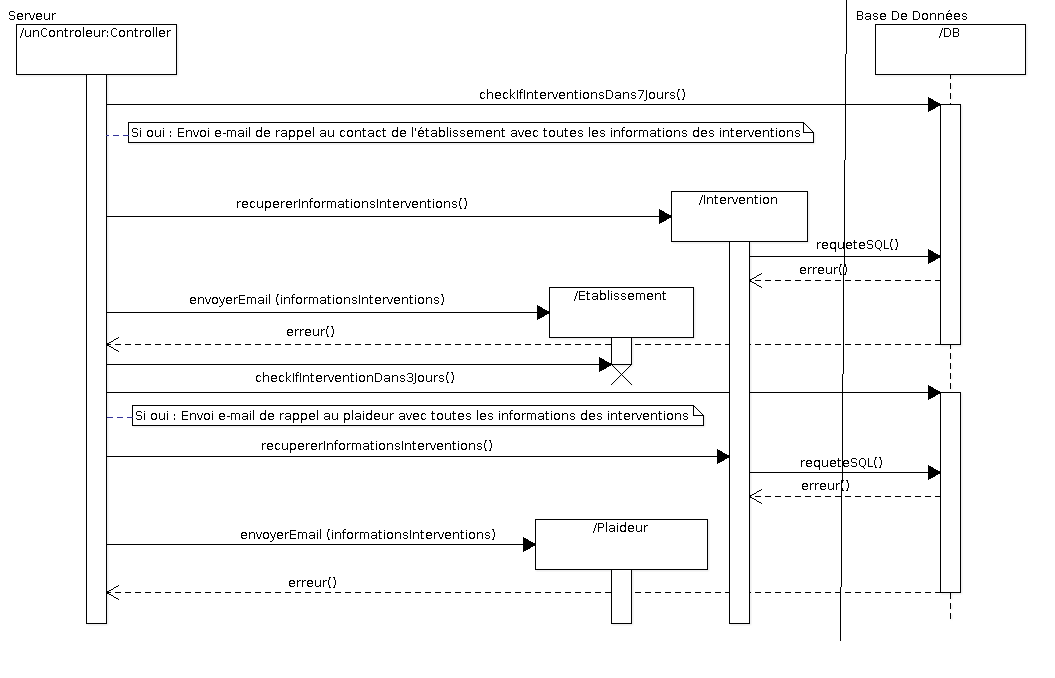
\includegraphics[scale=0.5]{../../lot2/DCP/images/diagrammesInteraction/07_diagrammeInteractionF5.png}
	\caption{Diagramme d'intération~: Géolocalisation des interventions et affectation à une intervention}
	\label{diagrammeInteraction7}
\end{figure}

\subsection{Fonctionnalité 6}
Ce paragraphe décrit le diagramme d'intéraction concernant la fonctionnalité 6. \\

La figure suivante (figure \ref{diagrammeInteraction8}) indique le déroulement de la mise à jour du planning d'un plaideur et l'information de prise en charge de l'intervention à l'établissement.
\begin{figure}[H]
	\centering
	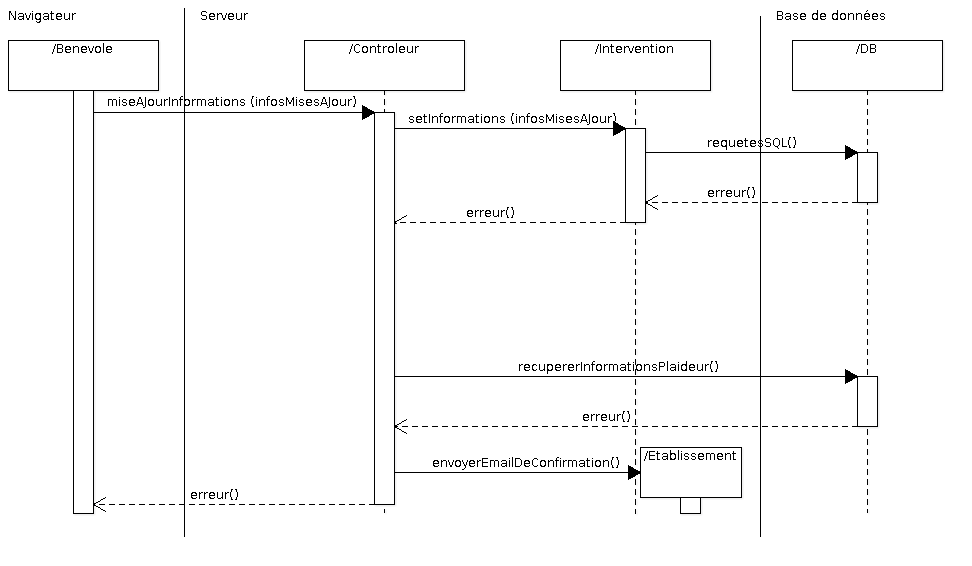
\includegraphics[scale=0.5]{../../lot2/DCP/images/diagrammesInteraction/08_diagrammeInteractionF6.png}
	\caption{Diagramme d'intéraction~: Mise à jour du planning d'un plaideur et information à l'établissement}
	\label{diagrammeInteraction8}
\end{figure}




\subsection{Fonctionnalité 7}
Ce paragraphe décrit le diagramme d'intéraction concernant la fonctionnalité 7.\\

La figure suivante (figure \ref{diagrammeInteraction9}) indique le déroulement de l'envoi des emails de rappel au plaideur et à l'établissement.
\begin{figure}[H]
	\centering
	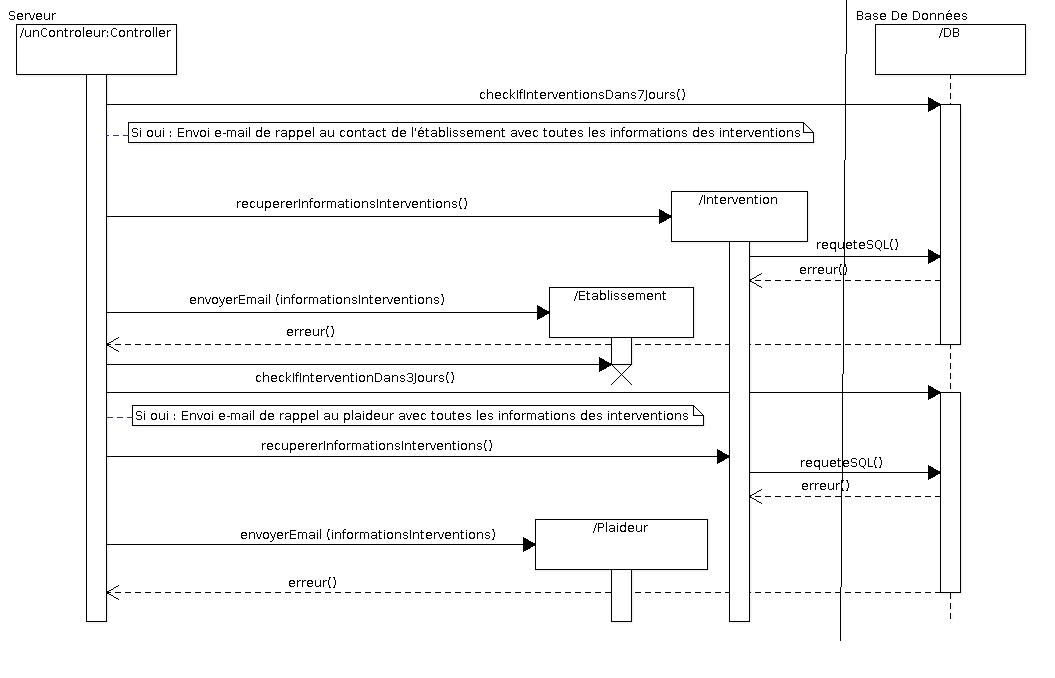
\includegraphics[scale=0.5]{../../lot2/DCP/images/diagrammesInteraction/09_diagrammeInteractionF7.png}
	\caption{Diagramme intéraction~: Envoi des emails de rappel}
	\label{diagrammeInteraction9}
\end{figure}

\section{Lot 3}
\subsection{Fonctionnalité 8}
Ce paragraphe décrit le diagramme d'intéraction concernant la fonctionnalité 8 soit la géolocalisation. \\

La figure suivant (figure \ref{diagrammeInteraction1}) indique le déroulement de la consultation d'une entité possédant une adresse.
\begin{figure}[H]
	\centering
	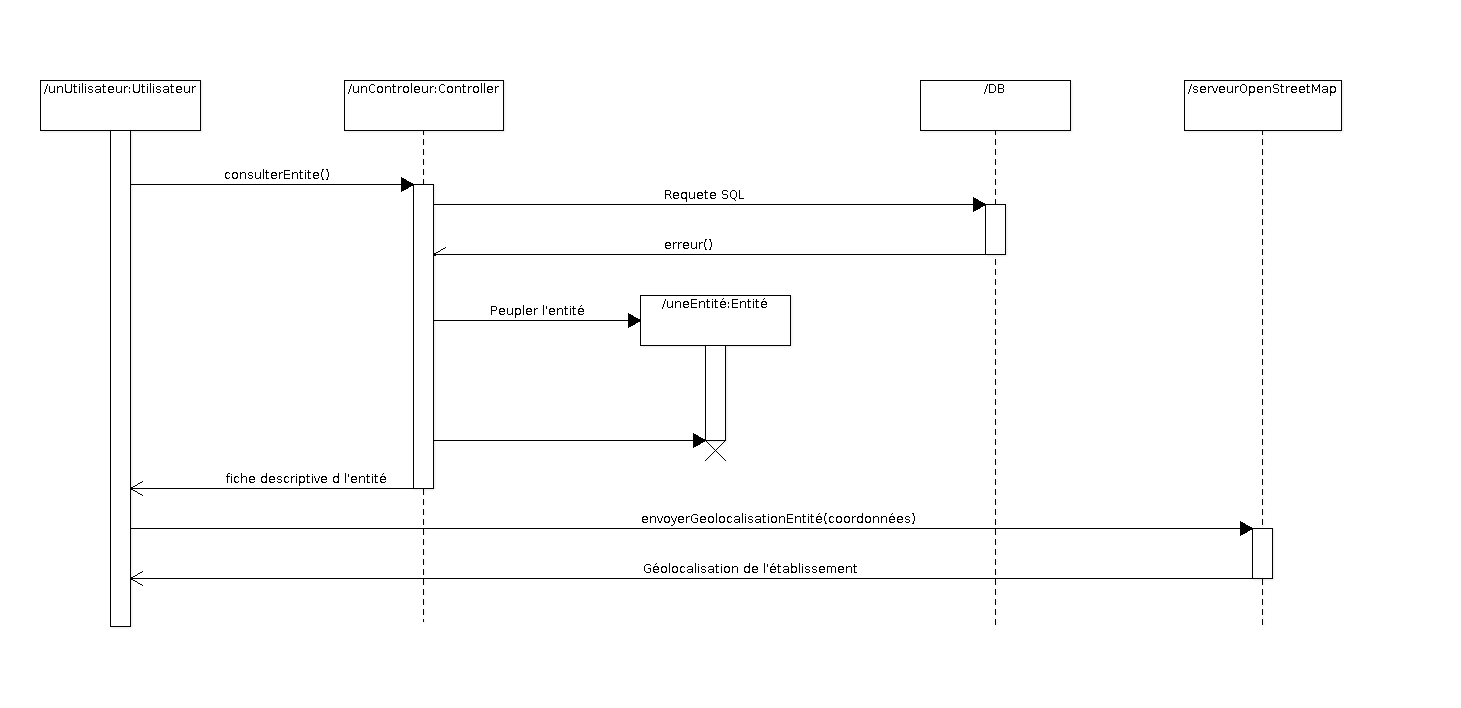
\includegraphics[scale=0.39]{images/diagrammesInteraction/01_diagrammeInteractionF8.png}
	\caption{Diagramme d'intéraction~: consultation d'une entité possédant une adresse}
	\label{diagrammeInteraction1}
\end{figure}

\subsection{Fonctionnalité 9}
Ce paragraphe décrit le diagramme d'intéraction concernant la fonctionnalité 9 soit l'attribution de frimousse. \\

La figure suivante (figure \ref{diagrammeInteraction3}) indique le déroulement de l'attribution d'une intervention de type frimousse.
\begin{figure}[H]
	\centering
	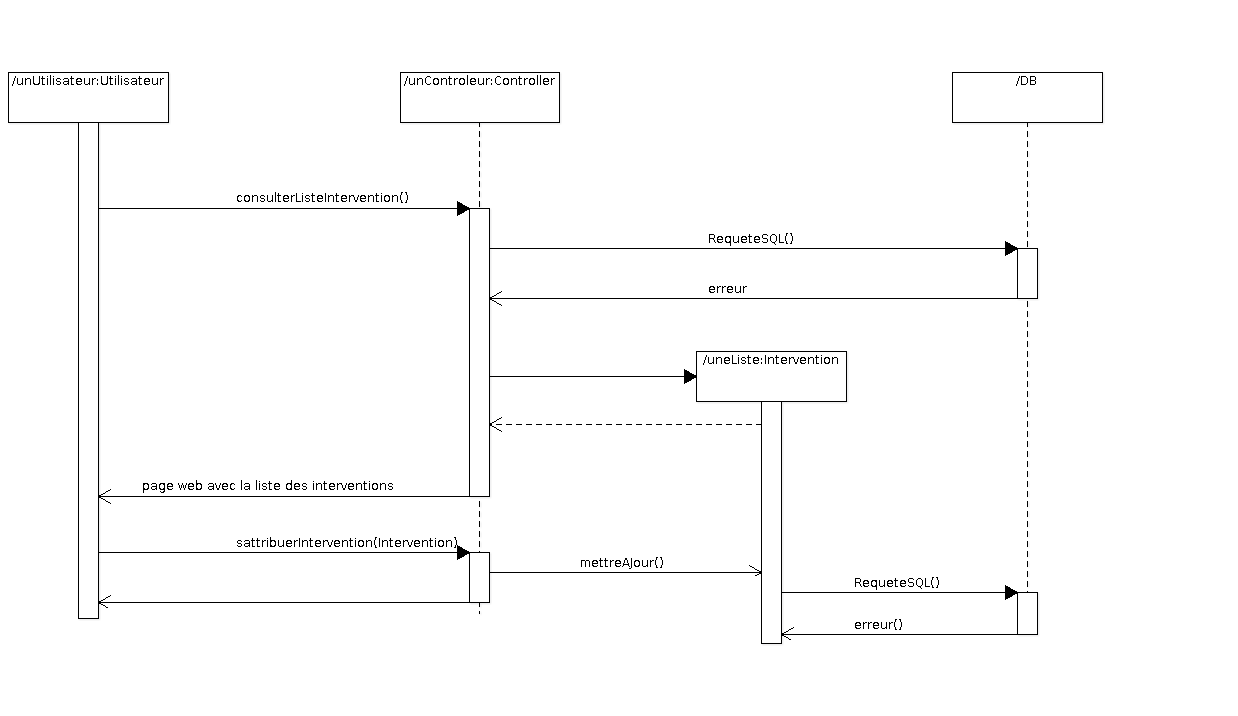
\includegraphics[scale=0.45]{images/diagrammesInteraction/02_diagrammeInteractionF9.png}
	\caption{Diagramme d'intéraction~: attribution d'une intervention de type frimousse }
	\label{diagrammeInteraction3}
\end{figure}

\subsection{Fonctionnalité 10}
Ce paragraphe décrit le diagramme d'intéraction concernant la fonctionnalité 10 soit la gestion des ventes. \\

La figure suivante (figure \ref{diagrammeInteraction3}) indique le déroulement de la création, modification, suppression d’une vente par un utilisateur. Il est à noter que seules les administrateurs auront la possibilité de supprimer une vente.
\begin{figure}[H]
	\centering
	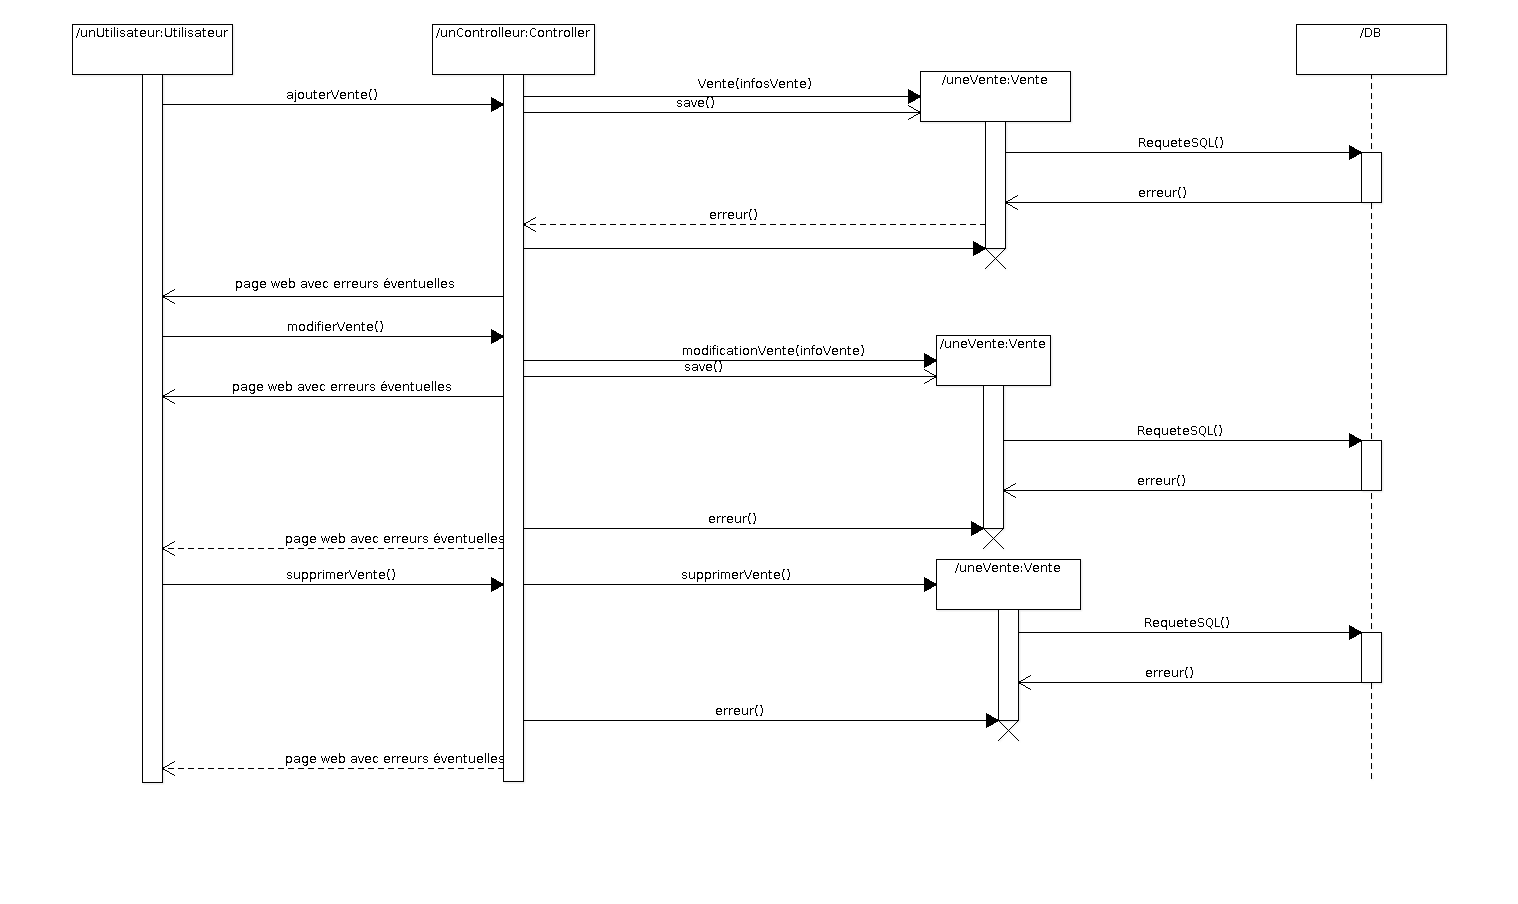
\includegraphics[scale=0.35]{images/diagrammesInteraction/03_diagrammeInteractionF10.png}
	\caption{Diagramme d'intéraction~: Création, modification, suppression d’une vente par un utilisateur}
	\label{diagrammeInteraction3}
\end{figure}


\section{Lot 4}
\subsection{Fonctionnalité 11}
Ce paragraphe décrit le diagramme d'intéraction concernant la fonctionnalité 11 soit la gestion des statistiques. \\

La figure suivante (figure \ref{diagrammeInteraction4}) indique le déroulement de la consultation des statistiques. 
\begin{figure}[H]
	\centering
	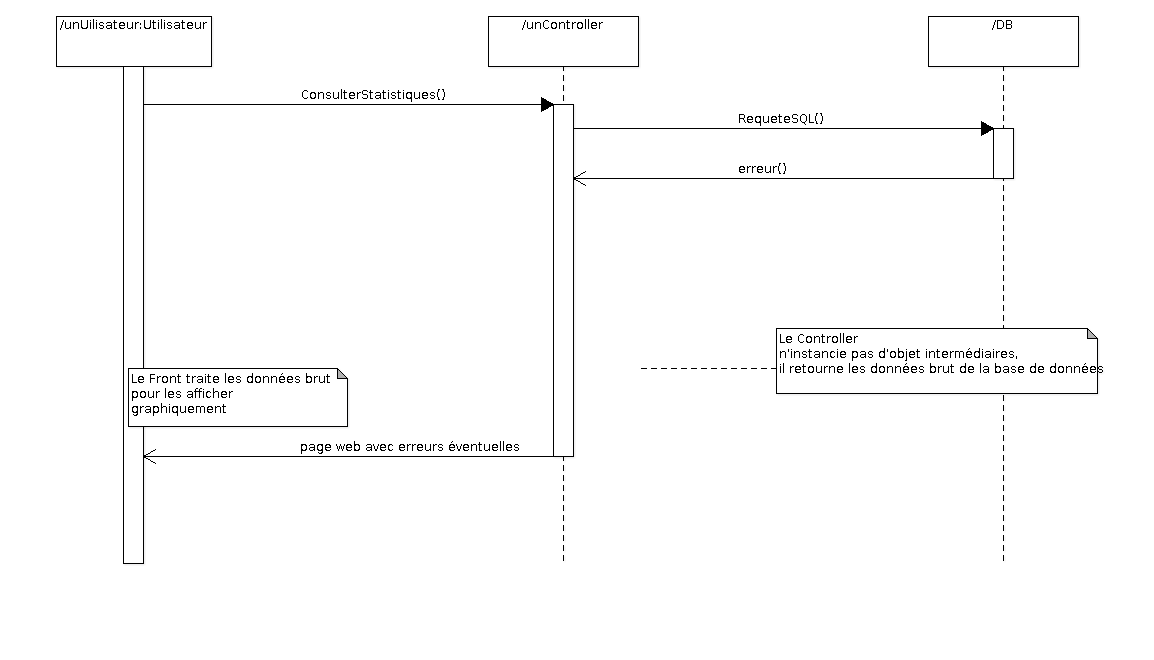
\includegraphics[scale=0.35]{images/diagrammesInteraction/04_diagrammeInteractionF11.png}
	\caption{Diagramme d'intéraction~: Consulter les statistiques}
	\label{diagrammeInteraction4}
\end{figure}


\chapter{Diagramme de classes de conception préliminaire}
\label{diagrammeClasses}
Ce chapitre décrit le diagramme de classe de conception préliminaire.

La figure suivante (figure \ref{diagrammeClasse}) présente le diagramme de classe de conception préliminaire.
\begin{figure}[H]
	\centering
	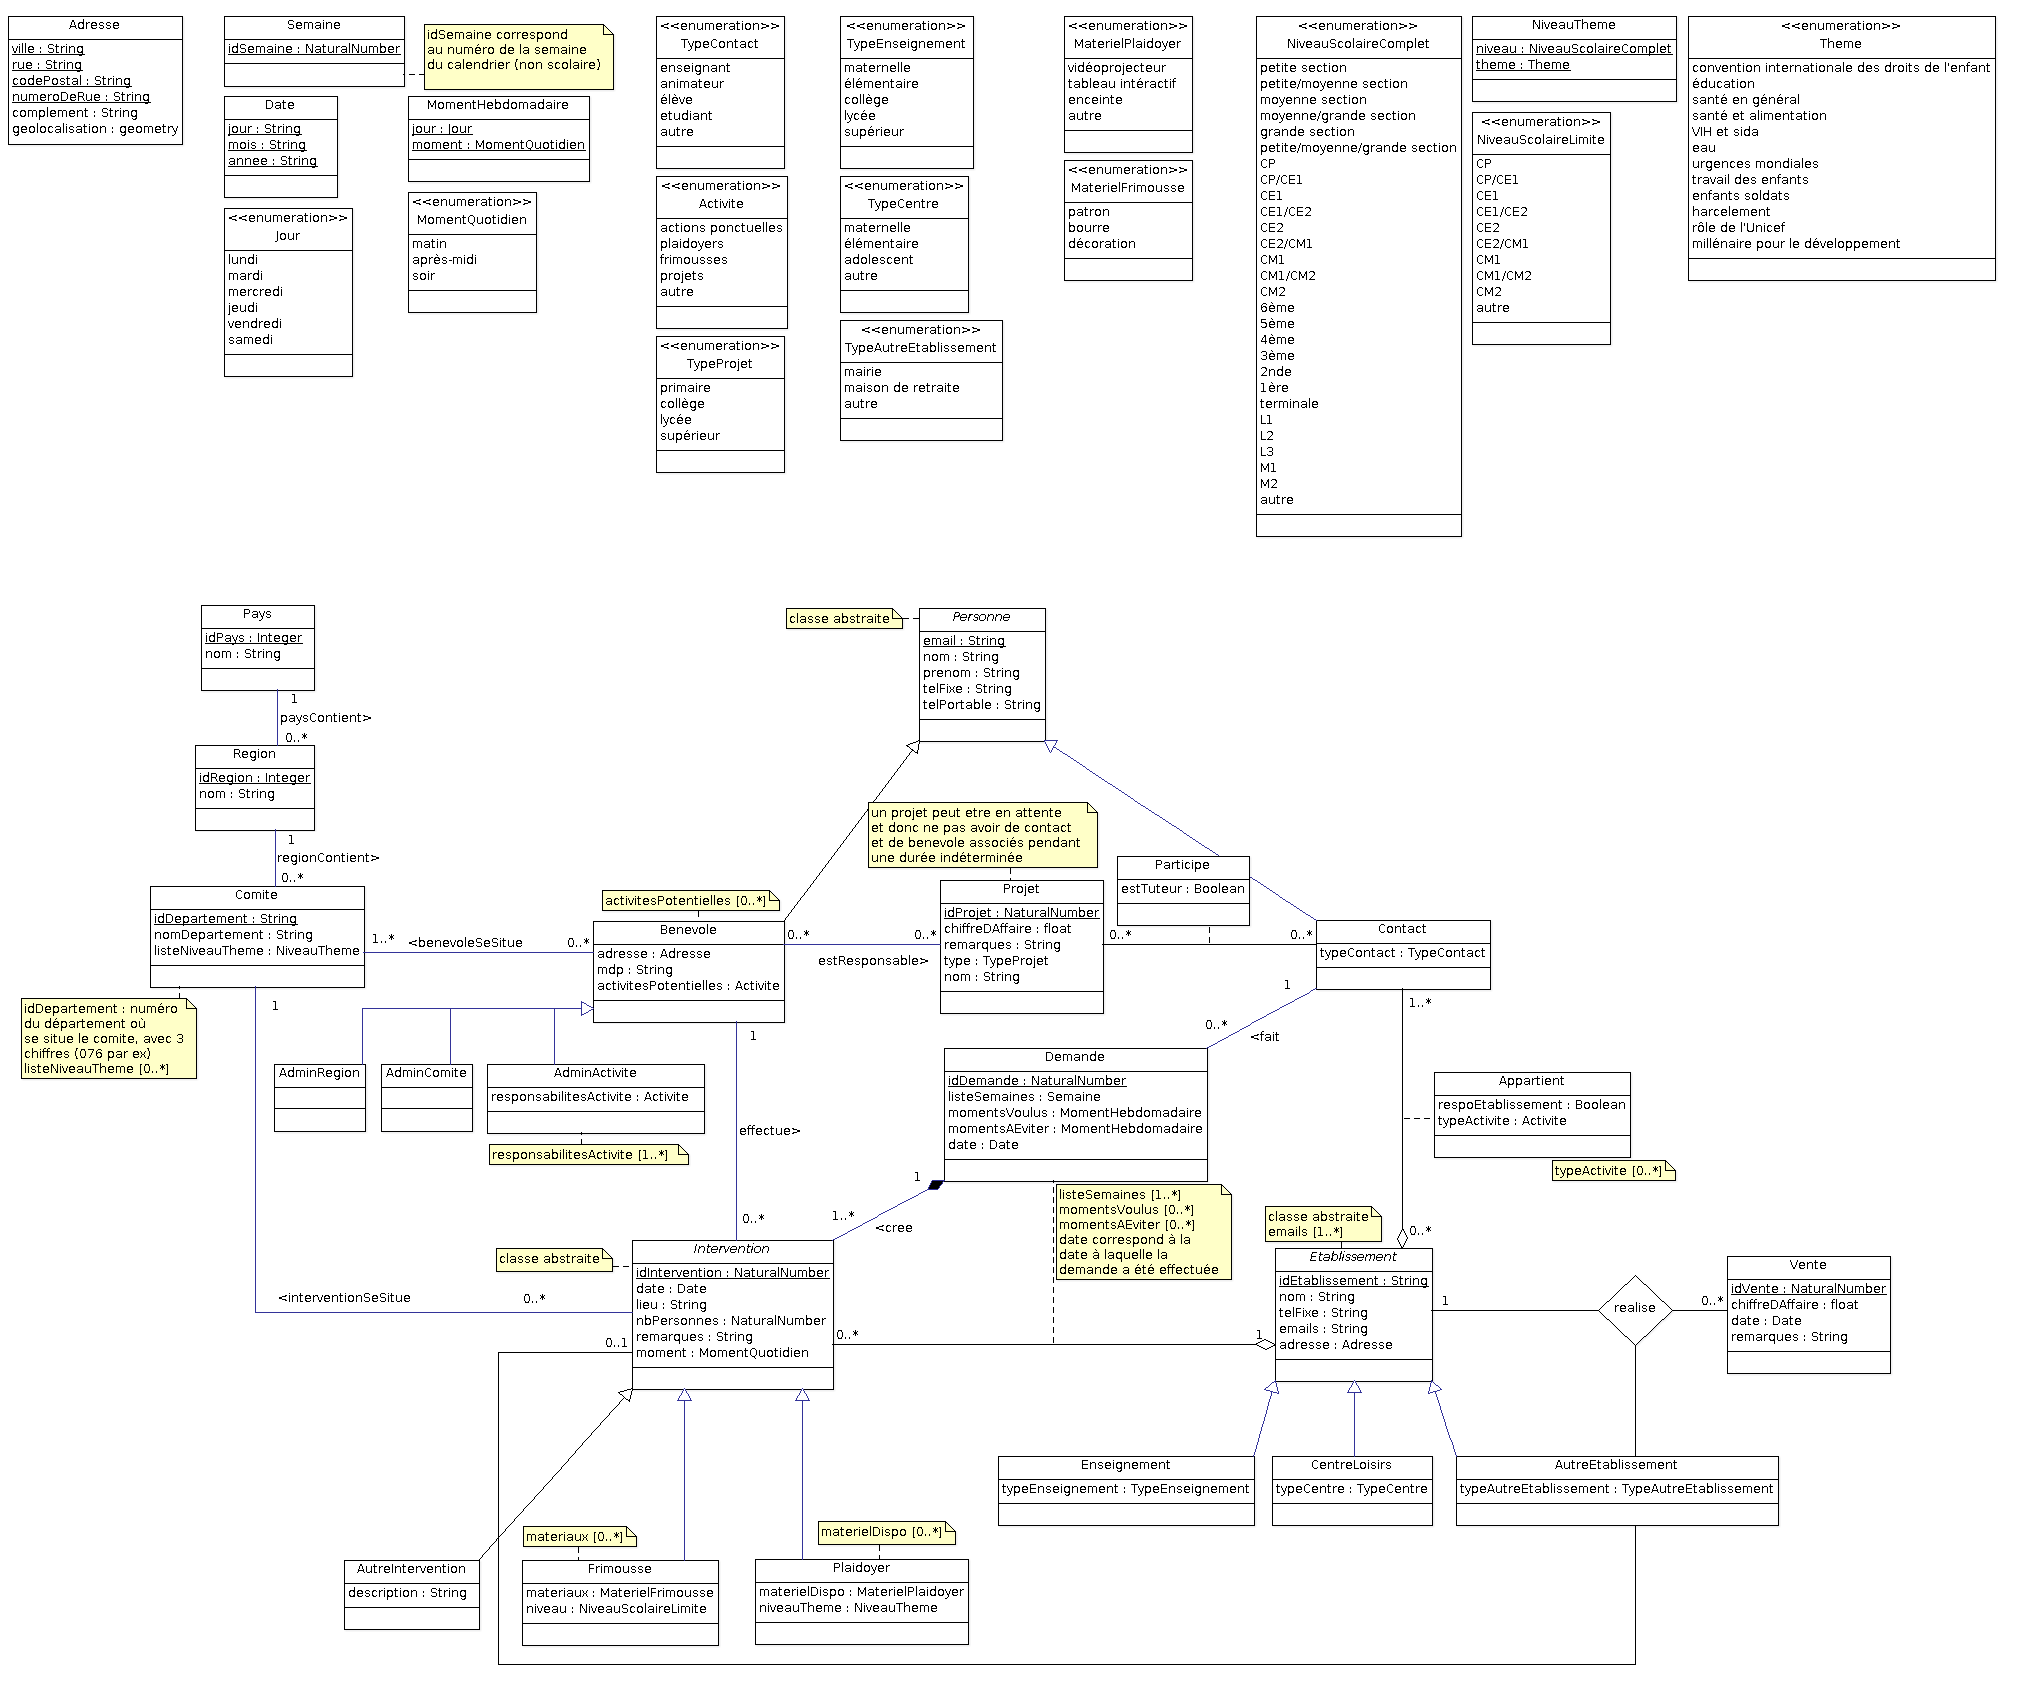
\includegraphics[scale=0.25]{images/diagrammeClasses/images/diagrammeDeClasses.png}
	\caption{Diagramme de classe de conception préliminaire}
	\label{diagrammeClasse}
	Le Dictionnaire de données permettant de décrire le diagramme de classes est situé en Annexe \ref{dico_donnees} 
\end{figure}

\chapter{Découpage en packages et leur signature}
\label{diagrammePackages}
Ce chapitre décrit le diagramme de packages.

La figure suivante (figure \ref{diagrammePackages}) présente le diagramme de packages.
\begin{figure}[H]
	\centering
	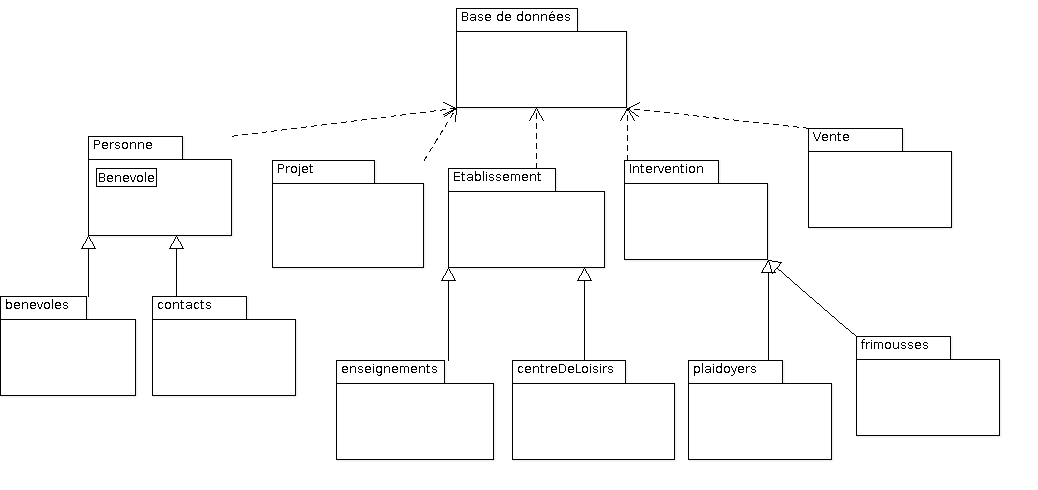
\includegraphics[scale=0.12]{images/diagrammePackages/diagrammeDePackages.png}
	\caption{Diagramme de packages}
	\label{diagrammePackages}
\end{figure}

\begin{appendix}
\part*{Annexes}
\addcontentsline{toc}{part}{Annexes}

\listoffigures
\addcontentsline{toc}{chapter}{Table des figures}
	 
\listoftables
\addcontentsline{toc}{chapter}{Liste des tableaux}
\end{appendix}
\pageQuatriemeCouverture

\end{document}